%%%%%%%%%%%%%%%%%%%%%%%%%%%%%%%%%%%%%%%%%%%%%%%%%%%%%%%
% MatPlotLib and Random Cheatsheet
%
% Edited by Maverick Lin
%
%%%%%%%%%%%%%%%%%%%%%%%%%%%%%%%%%%%%%%%%%%%%%%%%%%%%%%%
\documentclass[9pt]{extarticle}
% \documentclass{article}
\usepackage[landscape]{geometry}
\usepackage{url}
\usepackage{multicol}
\usepackage{amsmath}
\usepackage{amsfonts}
\usepackage{tikz}
\usetikzlibrary{decorations.pathmorphing}
\usepackage{amsmath,amssymb}

\usepackage{colortbl}
\usepackage{xcolor}
\usepackage{mathtools}
\usepackage{amsmath,amssymb}
\usepackage{enumitem}
\usepackage{tabto}
\usepackage{enumitem}
\usepackage{graphicx}
\usepackage{tabu}

\title{Data Science Cheat Sheet}
\usepackage[brazilian]{babel}
\usepackage[utf8]{inputenc}

\advance\topmargin-.8in
\advance\textheight3in
\advance\textwidth3in
\advance\oddsidemargin-1.5in
\advance\evensidemargin-1.5in
\parindent0pt
\parskip2pt
\newcommand{\hr}{\centerline{\rule{3.5in}{1pt}}}
%\colorbox[HTML]{e4e4e4}{\makebox[\textwidth-2\fboxsep][l]{texto}
\begin{document}

\begin{center}{\huge{\textbf{Data Science Cheatsheet}}}\\
{\large Compiled by Maverick Lin (\url{http://mavericklin.com})}\\
{\normalsize Last Updated August 10, 2018}
\end{center}
\begin{multicols*}{3}

\tikzstyle{mybox} = [draw=black, fill=white, very thick, rectangle, rounded corners, inner sep=10pt, inner ysep=10pt]
\tikzstyle{fancytitle} =[fill=black, text=white, font=\bfseries]
%------------ What is Data Science? ---------------
\begin{tikzpicture}
\node [mybox] (box){%
    \begin{minipage}{0.3\textwidth}
	Multi-disciplinary field that brings together concepts from computer science, statistics/machine learning, and data analysis to understand and extract insights from the ever-increasing amounts of data.\\
        
	Two paradigms of data research.
    \setlist{nolistsep}
    \begin{enumerate}[noitemsep]
  		\item \textbf{Hypothesis-Driven:} Given a problem, what kind of data do we need to help solve it?
  		\item \textbf{Data-Driven:} Given some data, what interesting problems can be solved with it?\\
	\end{enumerate}
    
    The heart of data science is to always ask questions. Always be curious about the world.
    \begin{enumerate}[noitemsep]
  		\item What can we learn from this data?
  		\item What actions can we take once we find whatever it is we are looking for?
	\end{enumerate}
    
    
    \end{minipage}
};
\node[fancytitle, right=10pt] at (box.north west) {What is Data Science?};
\end{tikzpicture}


%------------ Types of Data ---------------
\begin{tikzpicture}
\node [mybox] (box){%
    \begin{minipage}{0.3\textwidth}
		\textbf{Structured:} Data that has predefined structures. e.g. tables, spreadsheets, or relational databases.\\
        \textbf{Unstructured Data}: Data with no predefined structure, comes in any size or form, cannot be easily stored in tables. e.g. blobs of text, images, audio\\ 
        \textbf{Quantitative Data:} Numerical. e.g. height, weight\\
        \textbf{Categorical Data:} Data that can be labeled or divided into groups. e.g. race, sex, hair color.\\
        \textbf{Big Data:} Massive datasets, or data that contains greater \textit{variety} arriving in increasing \textit{volumes} and with ever-higher \textit{velocity} (3 Vs). Cannot fit in the memory of a single machine.\\
        
        {\color{blue} \textbf{Data Sources/Fomats}}\\
        \textbf{Most Common Data Formats} CSV, XML, SQL, JSON, Protocol Buffers\\
    	\textbf{Data Sources} Companies/Proprietary Data, APIs, Government, Academic, Web Scraping/Crawling

    \end{minipage};

};
\node[fancytitle, right=10pt] at (box.north west) {Types of Data};
\end{tikzpicture}


%------------ Main Types of Problems -----------------
\begin{tikzpicture}
\node [mybox] (box){%
    \begin{minipage}{0.3\textwidth}
    Two problems arise repeatedly in data science.\\
    \textbf{Classification:} Assigning something to a discrete set of possibilities. e.g. spam or non-spam, Democrat or Republican, blood type (A, B, AB, O) \\
    \textbf{Regression:} Predicting a numerical value. e.g. someone's income, next year GDP, stock price
    \end{minipage}
};
\node[fancytitle, right=10pt] at (box.north west) {Main Types of Problems};
\end{tikzpicture}


%------------ Probability Overview -------------------
\begin{tikzpicture}
\node [mybox] (box){%
    \begin{minipage}{0.3\textwidth}
	Probability theory provides a framework for reasoning about likelihood of events.\\
    \newline
    {\color{blue} \textbf{Terminology}}\\
    \textbf{Experiment:} procedure that yields one of a possible set of outcomes e.g. repeatedly tossing a die or coin \\
    \textbf{Sample Space S:} set of possible outcomes of an experiment e.g. if tossing a die, S = {(1,2,3,4,5,6}\\
    \textbf{Event E:} set of outcomes of an experiment e.g. event that a roll is 5, or the event that sum of 2 rolls is 7\\
    \textbf{Probability of an Outcome s or P(s):} number that satisfies 2 properties
	\setlist{nolistsep}	
    \begin{enumerate}[noitemsep]
  		\item for each outcome s, 0 $\leq$ P(s) $\leq$ 1
  		\item $\sum$ p(s) = 1\\
	\end{enumerate} 
    \textbf{Probability of Event E:} sum of the probabilities of the outcomes of the experiment: p(E) = $\sum_{s\subset E}$ p(s)\\
    \textbf{Random Variable V:} numerical function on the outcomes of a probability space\\
    \textbf{Expected Value of Random Variable V:} E(V) = $\sum_{s\subset S}$ p(s) * V(s)\\
    
    {\color{blue} \textbf{Independence, Conditional, Compound}}\\
    \textbf{Independent Events:} A and B are independent iff:\\
    	\centerline{P(A $\cap $ B) = P(A)P(B)}\\
        \centerline{P($A|B$) = P(A)}\\
        \centerline{P($B|A$) = P(B)}\\
    \textbf{Conditional Probability:} P($A|B$) = P(A,B)/P(B)\\
    \textbf{Bayes Theorem:} P($A|B$) = P($B|A$)P(A)/P(B)\\
    \textbf{Joint Probability:} P(A,B) = P($B|A$)P(A)\\
    \textbf{Marginal Probability:} P(A)\\
    
    {\color{blue} \textbf{Probability Distributions}}\\
    \textbf{Probability Density Function (PDF)} Gives the probability that a rv takes on the value x: $p_{X}(x) = P(X=x)$\\
    \textbf{Cumulative Density Function (CDF}) Gives the probability that a random variable is less than or equal to x: $F_{X}(x) = P(X\leq x)$\\
    \textit{Note}: The PDF and the CDF of a given random variable contain exactly the same information.

    \end{minipage}
};
\node[fancytitle, right=10pt] at (box.north west) {Probability Overview};
\end{tikzpicture}


%------------ Descriptive Statistics ---------------------
\begin{tikzpicture}
\node [mybox] (box){%
    \begin{minipage}{0.3\textwidth}
    	Provides a way of capturing a given data set or sample. There are two main types: \textbf{centrality} and \textbf{variability} measures.\\
     \newline 
    {\color{blue} \textbf{Centrality}}\\
	\textbf{Arithmetic Mean} Useful to characterize symmetric distributions without outliers $\mu_{X} = \frac{1}{n} \sum x$\\
	\textbf{Geometric Mean} Useful for averaging ratios. Always less than arithmetic mean =$\sqrt[\leftroot{-2}\uproot{2}n]{a_{1}a_{2}...a_{3}}$\\
    \textbf{Median} Exact middle value among a dataset. Useful for skewed distribution or data with outliers.\\
  	\textbf{Mode} Most frequent element in a dataset.\\
    
    {\color{blue} \textbf{Variability}}\\
	\textbf{Standard Deviation } Measures the squares differences between the individual elements and the mean\\
    \centerline{$\sigma = \sqrt{\frac{\sum_{i=1}^N (x_i - \overline{x})^2}{N-1}}$}\\
    \textbf{Variance} V = $\sigma^2$\\
    
%    	{\color{blue} \textbf{Characterizing Distributions}}\\
%     Taken together, the mean and the standard deviation can characterize any distribution. Good practice to report both mean and standard deviation to characterize your distribution: $\mu \pm \sigma$\\

    
    
    {\color{blue} \textbf{Interpreting Variance}}\\
    Variance is an inherent part of the universe. It is impossible to obtain the same results after repeated observations of the same event due to random noise/error. Variance can be explained away by attributing to sampling or measurement errors. Other times, the variance is due to the random fluctuations of the universe.\\
    
    {\color{blue} \textbf{Correlation Analysis}}
   
    Correlation coefficients r(X,Y) is a statistic that measures the degree that Y is a function of X and vice versa. Correlation values range from -1 to 1, where 1 means fully correlated, -1 means negatively-correlated, and 0 means no correlation.\\
    \textbf{Pearson Coefficient} Measures the degree of the relationship between linearly related variables\\
    \centerline{r = $\frac{Cov(X,Y)}{\sigma(X)\sigma(Y)}$}\\
    \textbf{Spearman Rank Coefficient} Computed on ranks and depicts monotonic relationships\\
    
    \textit{Note:} Correlation does not imply causation!
    \end{minipage}
};
\node[fancytitle, right=10pt] at (box.north west) {Descriptive Statistics};
\end{tikzpicture}

\newpage
% ------------ Data Cleaning----------------
\begin{tikzpicture}
\node [mybox] (box){%
    \begin{minipage}{0.3\textwidth}
	Data Cleaning is the process of turning raw data into a clean and analyzable data set. "Garbage in, garbage out." Make sure garbage doesn't get put in.\\
    
    {\color{blue} \textbf{Errors vs. Artifacts}}
   	\setlist{nolistsep}	
    \begin{enumerate}[noitemsep]
  		\item \textbf{Errors:} information that is lost during acquisition and can never be recovered e.g. power outage, crashed servers
  		\item \textbf{Artifacts:} systematic problems that arise from the data cleaning process. these problems can be corrected but we must first discover them\\
	\end{enumerate}
    
    {\color{blue} \textbf{Data Compatibility}}\\
    Data compatibility problems arise when merging datasets. Make sure you are comparing "apples to apples" and not "apples to oranges". Main types of conversions/unifications: 
    
    \begin{itemize}[noitemsep]
    	\item \textbf{units} (metric vs. imperial)
        \item \textbf{numbers} (decimals vs. integers), 
        \item \textbf{names} (John Smith vs. Smith, John),
        \item \textbf{time/dates} (UNIX vs. UTC vs. GMT), 
        \item \textbf{currency} (currency type, inflation-adjusted, dividends)\\
    \end{itemize}
    
    {\color{blue} \textbf{Data Imputation}}\\
    Process of dealing with missing values. The proper methods depend on the type of data we are working with. General methods include:
    
    \begin{itemize}[noitemsep]
    	\item Drop all records containing missing data
        \item Heuristic-Based: make a reasonable guess based on knowledge of the underlying domain
        \item Mean Value: fill in missing data with the mean
        \item Random Value
        \item Nearest Neighbor: fill in missing data using similar data points
        \item Interpolation: use a method like linear regression to predict the value of the missing data\\
    \end{itemize}
    
    \textbf{Outlier Detection} Outliers can interfere with analysis and often arise from mistakes during data collection. It makes sense to run a "sanity check".\\
    
    \textit{Note:} When cleaning data, always maintain both the raw data and the cleaned version(s). The raw data should be kept intact and preserved for future use. Any type of data cleaning/analysis should be done on a copy of the raw data. 
    \end{minipage}
};
\node[fancytitle, right=10pt] at (box.north west) {Data Cleaning};
\end{tikzpicture}



%------------ Statistical Analysis -----------------
\begin{tikzpicture}
\node [mybox] (box){%
    \begin{minipage}{0.3\textwidth}
    	Process of statistical reasoning: there is an underlying population of possible things we can potentially observe and only a small subset of them are actually sampled (ideally at random). Probability theory describes what properties our sample should have given the properties of the population, but \textbf{\textit{statistical inference}} allows us to deduce what the full population is like after analyzing the sample.
		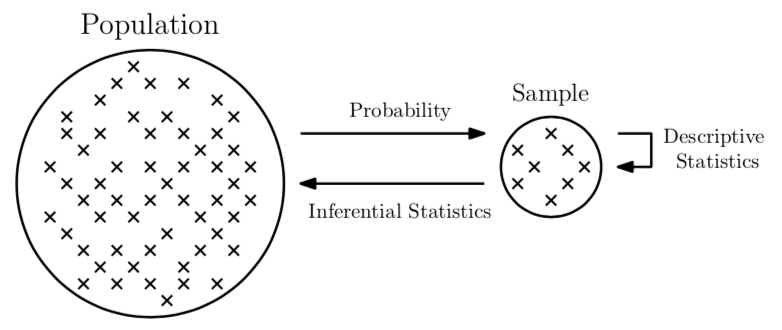
\includegraphics[width=\linewidth]{Figures/Central_Dogma_Statistics.png}
        
        {\color{blue} \textbf{Sampling From Distributions}}\\
        \textbf{Inverse Transform Sampling} Sampling points from a given probability distribution is sometimes necessary to run simulations or whether your data fits a particular distribution. The general technique is called \textit{inverse transform sampling} or Smirnov transform. First draw a random number \textit{p} between [0,1]. Compute value x such that the CDF equals \textit{p}: $F_{X}(x)$ = \textit{p}. Use x as the value to be the random value drawn from the distribution described by $F_{X}(x)$.\\
        \newline
        \textbf{Monte Carlo Sampling} In higher dimensions, correctly sampling from a given distribution becomes more tricky. Generally want to use Monte Carlo methods, which typically follow these rules: define  a domain of possible inputs, generate random inputs from a probability distribution over the domain, perform a deterministic calculation, and analyze the results. 
    \end{minipage}
};
\node[fancytitle, right=10pt] at (box.north west) {Statistical Analysis};
\end{tikzpicture}


%------------ Statistical Distributions -----------------
\begin{tikzpicture}
\node [mybox] (box){%
    \begin{minipage}{0.3\textwidth}
        \textbf{Binomial Distribution} (Discrete)\\
        Assume X is distributed Bin(n,p). X is the number of "successes" that we will achieve in n independent trials, where each trial is either a success or failure and each success occurs with the same probability p and each failure occurs with probability q=1-p.\\
        PDF: $P(X=x) =  \binom{n}{k} p^x (1-p)^{n-x}$\\
        EV: $\mu = np$ \space\space Variance = npq
        \newline
        
        \textbf{Normal/Gaussian Distribution} (Continuous)\\
        Assume X in distributed $\mathcal{N}(\mu,\,\sigma^{2})$. It is a bell-shaped and symmetric distribution. Bulk of the values lie close to the mean and no value is too extreme. Generalization of the binomial distribution as n $\to \infty$.\\
        PDF: $P(x) = \frac{1}{{\sigma \sqrt {2\pi } }}e^{{{ - \left( {x - \mu } \right)^2 } \mathord{\left/ {\vphantom {{ - \left( {x - \mu } \right)^2 } {2\sigma ^2 }}} \right. \kern-\nulldelimiterspace} {2\sigma ^2 }}}$\\
        EV: $\mu$ \space\space Variance: $\sigma^2$\\
        \textbf{Implications}: 68\%-95\%-99\% rule. 68\% of probability mass fall within 1$\sigma$ of the mean, 95\% within 2$\sigma$, and 99.7\% within 3$\sigma$.\\

        \textbf{Poisson Distribution} (Discrete)\\
        Assume X is distributed Pois($\lambda$). Poisson expresses the probability of a given number of events occurring in a fixed interval of time/space if these events occur independently and with a known constant rate $\lambda$.\\
        PDF: $P\left( x \right) = \frac{{e^{ - \lambda } \lambda ^x }}{{x!}}$ \space\space EV: $\lambda$ \space\space Variance = $\lambda$\\
        \newline
        \textbf{Power Law Distributions} (Discrete)\\
        Many data distributions have much longer tails than the normal or Poisson distributions. In other words, the change in one quantity varies as a \textit{power} of another quantity. It helps measure the inequality in the world. e.g. wealth, word frequency and Pareto Principle (80/20 Rule) \\
        PDF: P(X=x) = c$x^{-\alpha}$, where $\alpha$ is the law's exponent and c is the normalizing constant
      	\begin{center}
    	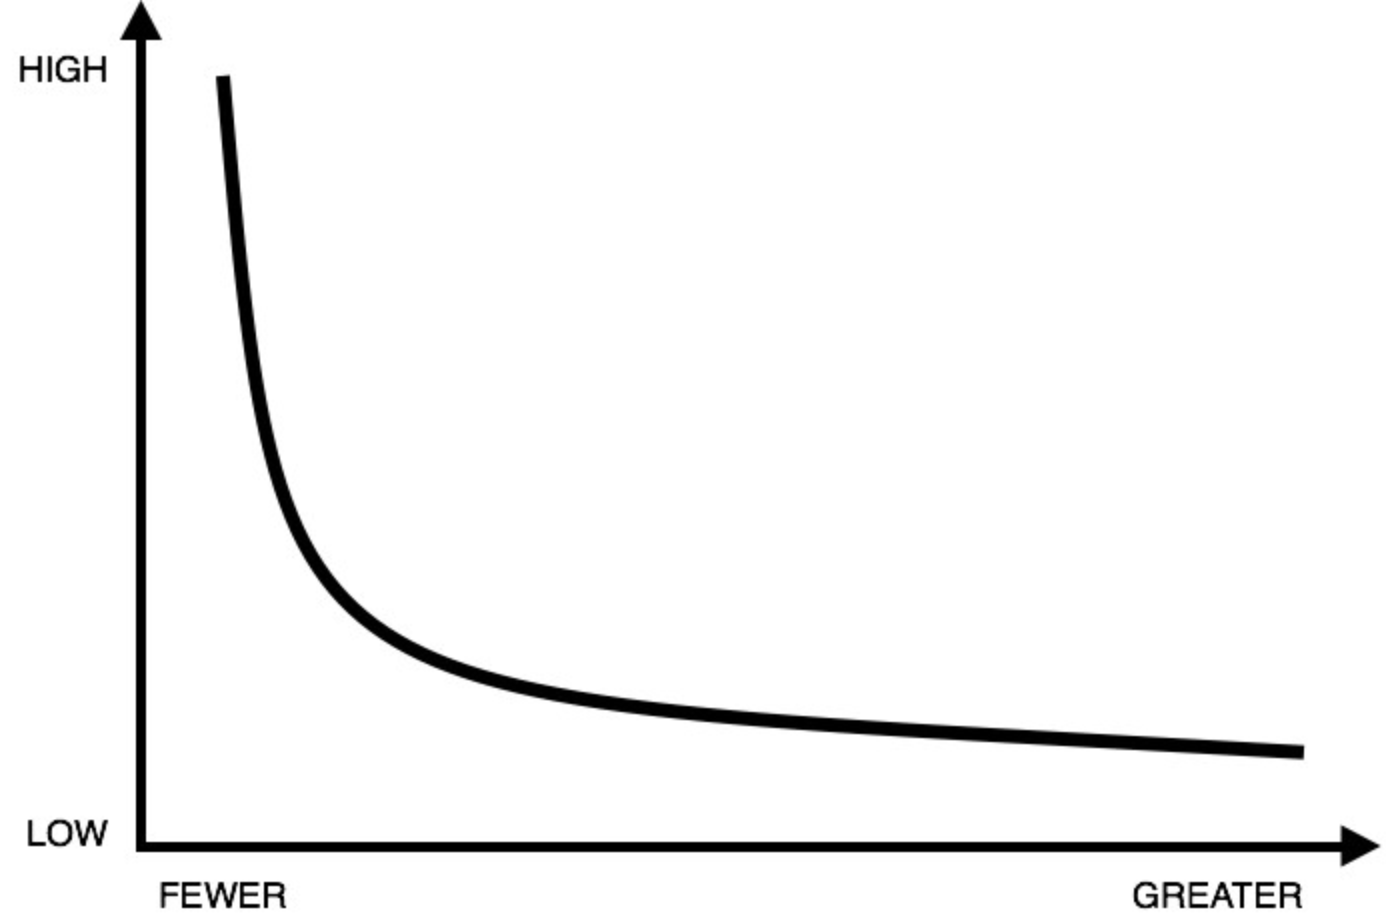
\includegraphics[width=5cm, height=3cm]{Figures/power-law.png}
		\end{center}
    \end{minipage}
};
\node[fancytitle, right=10pt] at (box.north west) {Classic Statistical Distributions};
\end{tikzpicture}


% ------------ Modeling Overview -----------------
\begin{tikzpicture}
\node [mybox] (box){%
    \begin{minipage}{0.3\textwidth}
    Modeling is the process of incorporating information into a tool which can forecast and make predictions. Usually, we are dealing with statistical modeling where we want to analyze relationships between variables. Formally, we want to estimate a function $f(X)$ such that:
    \begin{center}
    	$Y = f(X) + \epsilon$
    \end{center}
    where X = ($X_{1}, X_{2},...X_{p}$) represents the input variables, Y represents the output variable, and $\epsilon$ represents random error.\\
    
    \textit{\textbf{Statistical learning}} is set of approaches for estimating this $f(X)$. \\
    
    {\color{blue} \textbf{Why Estimate f(X)?}}\\
    \textbf{Prediction}: once we have a good estimate $\hat{f}(X)$, we can use it to make predictions on new data. We treat $\hat{f}$ as a black box, since we only care about the accuracy of the predictions, not why or how it works. \\
    \textbf{Inference}: we want to understand the relationship between X and Y. We can no longer treat $\hat{f}$ as a black box since we want to understand how Y changes with respect to X = ($X_{1}, X_{2},...X_{p}$)\\
        
        \setlist{nolistsep}	
        {\color{blue} \textbf{More About $\epsilon$}}\\
		The error term $\epsilon$ is composed of the reducible and irreducible error, which will prevent us from ever obtaining a perfect $\hat{f}$ estimate. 
        \begin{itemize}[noitemsep]
        	\item \textbf{Reducible}: error that can potentially be reduced by using the most appropriate statistical learning technique to estimate $f$. The goal is to minimize the reducible error.
            \item \textbf{Irreducible}: error that cannot be reduced no matter how well we estimate $f$. Irreducible error is unknown and unmeasurable and will always be an upper bound for $\epsilon$.\\
        \end{itemize}
        
     \textit{Note}: There will always be trade-offs between model flexibility (prediction) and model interpretability (inference). This is just another case of the bias-variance trade-off. Typically, as flexibility increases, interpretability decreases. Much of statistical learning/modeling is finding a way to balance the two.
    \end{minipage}
};
\node[fancytitle, right=10pt] at (box.north west) {Modeling- Overview};
\end{tikzpicture}


%------------ Modeling- Philosophies -----------------
\begin{tikzpicture}
\node [mybox] (box){%
    \begin{minipage}{0.3\textwidth}
    	Modeling is the process of incorporating information into a tool which can forecast and make predictions. Designing and validating models is important, as well as evaluating the performance of models. Note that the best forecasting model may not be the most accurate one.\\
        
        {\color{blue} \textbf{Philosophies of Modeling}}\\
        \textbf{Occam's Razor} Philosophical principle that the simplest explanation is the best explanation. In modeling, if we are given two models that predicts equally well, we should choose the simpler one. Choosing the more complex one can often result in overfitting.\\
        \textbf{Bias Variance Trade-Off} Inherent part of predictive modeling, where models with lower bias will have higher variance and vice versa. Goal is to achieve low bias and low variance.
        
        \setlist{nolistsep}	
        \begin{itemize}[noitemsep]
  		\item \textbf{\textit{Bias}}: error from incorrect assumptions to make target function easier to learn (high bias $\to$ missing relevant relations or underfitting)
  		\item \textbf{\textit{Variance}}: error from sensitivity to fluctuations in the dataset, or how much the target estimate would differ if different training data was used (high variance $\to$ modeling noise or overfitting)
		\end{itemize} 
    	
        \begin{center}
    		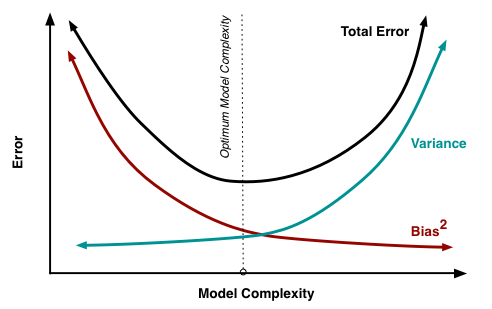
\includegraphics[width=5cm, height=3cm]{Figures/biasvariance.png}
		\end{center}
        
        \textbf{No Free Lunch Theorem} No single machine learning algorithm is better than all the others on all problems. It is common to try multiple models and find one that works best for a particular problem.\\

        
        {\color{blue} \textbf{Thinking Like Nate Silver}}\\
        \textbf{1. Think Probabilistically} Probabilistic forecasts are more meaningful than concrete statements and should be reported as probability distributions (including $\sigma$ along with mean prediction $\mu$.\\
        \textbf{2. Incorporate New Information} Use live models, which continually updates using new information. To update, use Bayesian reasoning to calculate how probabilities change in response to new evidence.\\
        \textbf{3. Look For Consensus Forecast} Use multiple distinct sources of evidence. Ssome models operate this way, such as boosting and bagging, which uses large number of weak classifiers to produce a strong one. 
    \end{minipage}
};
\node[fancytitle, right=10pt] at (box.north west) {Modeling- Philosophies};
\end{tikzpicture}


%------------ Modeling- Taxonomy -----------------
\begin{tikzpicture}
\node [mybox] (box){%
    \begin{minipage}{0.3\textwidth}
		There are many different types of models. It is important to understand the trade-offs and when to use a certain type of model.\\
        
        {\color{blue} \textbf{Parametric vs. Nonparametric}}
        \setlist{nolistsep}	
        \begin{itemize}[noitemsep]
  		\item \textbf{Parametric}: models that first make an assumption about a function form, or shape, of $f$ (linear). Then fits the model. This reduces estimating $f$ to just estimating set of parameters, but if our assumption was wrong, will lead to bad results.
  		\item \textbf{Non-Parametric}: models that don't make any assumptions about $f$, which allows them to fit a wider range of shapes; but may lead to overfitting
		\end{itemize} 
        
        {\color{blue} \textbf{Supervised vs. Unsupervised}}
        \setlist{nolistsep}	
        \begin{itemize}[noitemsep]
  		\item \textbf{Supervised}: models that fit input variables $x_{i} = (x_{1}, x_{2},...x_{n}$) to a known output variables $y_{i} = (y_{1}, y_{2},...y_{n}$)
  		\item \textbf{Unsupervised}: models that take in input variables $x_{i} = (x_{1}, x_{2},...x_{n}$), but they do not have an associated output to supervise the training. The goal is understand relationships between the variables or observations.
		\end{itemize} 
        
        {\color{blue} \textbf{Blackbox vs. Descriptive}}
        \setlist{nolistsep}	
        \begin{itemize}[noitemsep]
  		\item \textbf{Blackbox}: models that make decisions, but we do not know what happens "under the hood" e.g. deep learning, neural networks
  		\item \textbf{Descriptive}: models that provide insight into \textit{why} they make their decisions e.g. linear regression, decision trees
		\end{itemize} 
        
        {\color{blue} \textbf{First-Principle vs. Data-Driven}}
        \setlist{nolistsep}	
        \begin{itemize}[noitemsep]
  		\item \textbf{First-Principle}: models based on a prior belief of how the system under investigation works, incorporates domain knowledge (ad-hoc)
  		\item \textbf{Data-Driven}: models based on observed correlations between input and output variables
		\end{itemize} 
        
        {\color{blue} \textbf{Deterministic vs. Stochastic}}
        \setlist{nolistsep}	
        \begin{itemize}[noitemsep]
  		\item \textbf{Deterministic}: models that produce a single "prediction" e.g. yes or no, true or false
  		\item \textbf{Stochastic}: models that produce probability distributions over possible events
		\end{itemize} 
        
        {\color{blue} \textbf{Flat vs. Hierarchical}}
        \setlist{nolistsep}	
        \begin{itemize}[noitemsep]
  		\item \textbf{Flat}: models that solve problems on a single level, no notion of subproblems
  		\item \textbf{Hierarchical}: models that solve several different nested subproblems
		\end{itemize} 
    \end{minipage}
    
};
\node[fancytitle, right=10pt] at (box.north west) {Modeling- Taxonomy};
\end{tikzpicture}

%------------ Modeling- Evaluation -----------------
\begin{tikzpicture}
\node [mybox] (box){%
    \begin{minipage}{0.3\textwidth}
    	Need to determine how good our model is. Best way to assess models is out-of-sample predictions (data points your model has never seen).\\
        
        {\color{blue} \textbf{Classification}}
        
        \begin{center}
        \footnotesize
        \begin{tabular}{ |c|c|c| } 
         \hline
          & Predicted Yes & Predicted No \\ 
         \hline
         Actual Yes & True Positives (TP) & False Negatives (FN)  \\ 
         Actual No & False Positives (FP) & True Negatives (TN) \\ 
         \hline
        \end{tabular}
        \end{center}
        \textbf{Accuracy}: ratio of correct predictions over total predictions. Misleading when class sizes are substantially different. $accuracy = \frac{TP + TN}{TP + TN + FN + FP}$\\
        \textbf{Precision}: how often the classifier is correct when it predicts positive: $precision = \frac{TP}{TP + FP}$ \\
        \textbf{Recall}: how often the classifier is correct for all positive instances: $recall = \frac{TP}{TP + FN}$ \\
        \textbf{F-Score}: single measurement to describe performance: F = 2 $\cdot$ $\frac{\text{precision} \cdot \text{recall}}{\text{precision + recall}}$ \\
      	\textbf{ROC Curves}: plots true positive rates and false positive rates for various thresholds, or where the model determines if a data point is positive or negative (e.g. if $>$0.8, classify as positive). Best possible area under the ROC curve (AUC) is 1, while random is 0.5, or the main diagonal line.\\
%         \begin{center}
%         	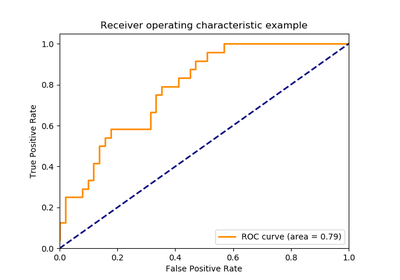
\includegraphics[width=5cm, height=3cm]{ROC.png}
%         \end{center}
        
        {\color{blue} \textbf{Regression}}\\
        Errors are defined as the difference between a prediction y$\prime$ and the actual result y.\\
        \textbf{Absolute Error}: $\Delta = y\prime - y$\\
        \textbf{Squared Error}: $\Delta^2 = (y\prime - y)^2$\\
        \textbf{Mean-Squared Error}: $MSE = \frac{1}{n}\sum_{i=1}^{n}(y\prime_{i} - y_i)^2$\\
        \textbf{Root Mean-Squared Error}: RMSD = $\sqrt{MSE}$\\
%         \textit{Note}: For squared errors, outliers have a disproportionate effect. \\
        \textbf{Absolute Error Distribution:} Plot absolute error distribution: should be symmetric, centered around 0, bell-shaped, and contain rare extreme outliers.
    \end{minipage}
};
\node[fancytitle, right=10pt] at (box.north west) {Modeling- Evaluation Metrics};
\end{tikzpicture}


% ------------ Modeling- Evaluation Environment-----------------
\begin{tikzpicture}
\node [mybox] (box){%
    \begin{minipage}{0.3\textwidth}
    	Evaluation metrics provides use with the tools to estimate errors, but what should be the process to obtain the best estimate? Resampling involves repeatedly drawing samples from a training set and refitting a model to each sample, which provides us with additional information compared to fitting the model once, such as obtaining a better estimate for the test error.\\
        
        {\color{blue} \textbf{Key Concepts}}\\
        \textbf{Training Data}: data used to fit your models or the set used for learning\\
        \textbf{Validation Data}: data used to tune the parameters of a model\\
        \textbf{Test Data}: data used to evaluate how good your model is. Ideally your model should never touch this data until final testing/evaluation\\
       
        {\color{blue} \textbf{Cross Validation}}\\
        Class of methods that estimate test error by holding out a subset of training data from the fitting process.\\
        \textbf{Validation Set}: split data into training set and validation set. Train model on training and estimate test error using validation. e.g. 80-20 split\\
        \textbf{Leave-One-Out CV (LOOCV)}: split data into training set and validation set, but the validation set consists of 1 observation. Then repeat n-1 times until all observations have been used as validation. Test erro is the average of these n test error estimates.\\
        \textbf{k-Fold CV}: randomly divide data into k groups (folds) of approximately equal size. First fold is used as validation and the rest as training. Then repeat k times and find average of the k estimates.\\
        
        {\color{blue} \textbf{Bootstrapping}}\\
        Methods that rely on random sampling with replacement. Bootstrapping helps with quantifying uncertainty associated with a given estimate or model.\\
        
        {\color{blue} \textbf{Amplifying Small Data Sets}}\\
        What can we do it we don't have enough data?
        \setlist{nolistsep}	

        \begin{itemize}[noitemsep]
        	\item \textbf{Create Negative Examples}- e.g. classifying presidential candidates, most people would be unqualified so label most as unqualified
            \item \textbf{Synthetic Data}- create additional data by adding noise to the real data
        \end{itemize}
    \end{minipage}
};
\node[fancytitle, right=10pt] at (box.north west) {Modeling- Evaluation Environment};
\end{tikzpicture}


% ------------ Machine Learning- Linear Regression -----------------
\begin{tikzpicture}
\node [mybox] (box){%
    \begin{minipage}{0.3\textwidth}
    Linear regression is a simple and useful tool for predicting a quantitative response. The relationship between input variables X = ($X_{1}, X_{2},...X_{p}$) and output variable Y takes the form:
    
    \begin{center}
    	$Y \approx \beta_{0} + \beta_{1}X_{1} + ... + \beta_{p}X_{p} + \epsilon$
    \end{center}
    
    $\beta_{0}...\beta_{p}$ are the unknown coefficients (parameters) which we are trying to determine. The best coefficients will lead us to the best "fit", which can be found by minimizing the \textit{residual sum squares} (RSS), or the sum of the differences between the actual $i$th value and the predicted $i$th value. RSS = $\sum_{i=1}^{n} e_{i}$, where $e_{i} = y_{i} - \hat{y_{i}}$\\
    
%     \begin{center}
    
%     \end{center}

    {\color{blue} \textbf{How to find best fit?}}\\
    \textbf{Matrix Form}: We can solve the closed-form equation for coefficient vector $w$: $w = (X^{T}X)^{-1}X^{T}Y$. X represents the input data and Y represents the output data. This method is used for smaller matrices, since inverting a matrix is computationally expensive.\\
    \textbf{Gradient Descent}: First-order optimization algorithm. We can find the minimum of a \textit{convex} function by starting at an arbitrary point and repeatedly take steps in the downward direction, which can be found by taking the negative direction of the gradient. After several iterations, we will eventually converge to the minimum. In our case, the minimum corresponds to the coefficients with the minimum error, or the best line of fit. The learning rate $\alpha$ determines the size of the steps we take in the downward direction.\\
    
    Gradient descent algorithm in two dimensions. Repeat until convergence.
    \setlist{nolistsep}	

    \begin{enumerate}
    	\item $w_0^{t+1} := w_0^{t} - \alpha \frac{\partial}{\partial w_0}J(w_0, w_1)$
        \item $w_1^{t+1} := w_1^{t} - \alpha \frac{\partial}{\partial w_1}J(w_0, w_1)$\\
    \end{enumerate}
    
    For non-convex functions, gradient descent no longer guarantees an optimal solutions since there may be local minimas. Instead, we should run the algorithm from different starting points and use the best local minima we find for the solution.\\
    \textbf{Stochastic Gradient Descent}: instead of taking a step after sampling the \textit{entire} training set, we take a small batch of training data at random to determine our next step. Computationally more efficient and may lead to faster convergence.
    \end{minipage}
};
\node[fancytitle, right=10pt] at (box.north west) {Linear Regression};
\end{tikzpicture}


% ------------ Linear Regression II -----------------
\begin{tikzpicture}
\node [mybox] (box){%
    \begin{minipage}{0.3\textwidth}
    
    {\color{blue} \textbf{Improving Linear Regression}}\\
    \textbf{Subset/Feature Selection}: approach involves identifying a subset of the $p$ predictors that we believe to be best related to the response. Then we fit model using the reduced set of variables.
    \setlist{nolistsep}	
    \begin{itemize}
	\item Best, Forward, and Backward Subset Selection
    \end{itemize}
    
    \textbf{Shrinkage/Regularization}: all variables are used, but estimated coefficients are shrunken towards zero relative to the least squares estimate. $\lambda$ represents the tuning parameter- as $\lambda$ increases, flexibility decreases $\to$ decreased variance but increased bias. The tuning parameter is key in determining the sweet spot between under and over-fitting. In addition, while Ridge will always produce a model with $p$ variables, Lasso can force coefficients to be equal to zero.
    	\begin{itemize}
        	\item Lasso (L1): min RSS + $\lambda \sum_{j=1}^{p}|\beta_j|$

        	\item Ridge (L2): min RSS + $\lambda \sum_{j=1}^{p}\beta_j^{2}$
        \end{itemize}
    \textbf{Dimension Reduction}: projecting $p$ predictors into a M-dimensional subspace, where M $<$ $p$. This is achieved by computing M different linear combinations of the variables. Can use PCA.\\
    \textbf{Miscellaneous}: Removing outliers, feature scaling, removing multicollinearity (correlated variables)\\
    
    {\color{blue} \textbf{Evaluating Model Accuracy}}\\
    Residual Standard Error (RSE): RSE = $\sqrt{\frac{1}{n-2}RSS}$. Generally, the smaller the better.\\
    $R^2$: Measure of fit that represents the proportion of variance explained, or the \textit{variability in Y that can be explained using X}. It takes on a value between 0 and 1. Generally the higher the better. $R^2 = 1 - \frac{RSS}{TSS}$, where Total Sum of Squares (TSS) = $\sum{(y_{i}-\bar{y})}^2$\\
    
    {\color{blue} \textbf{Evaluating Coefficient Estimates}}\\
    Standard Error (SE) of the coefficients can be used to perform hypothesis tests on the coefficients:\\
    $H_0$: No relationship between X and Y, $H_a$: Some relationship exists. A p-value can be obtained and can be interpreted as follows: a small p-value indicates that a relationship between the predictor (X) and the response (Y) exists. Typical p-value cutoffs are around 5 or 1 $\%$.
    
    \end{minipage}
};
\node[fancytitle, right=10pt] at (box.north west) {Linear Regression II};
\end{tikzpicture}


% ------------ Logistic Regression -----------------
\begin{tikzpicture}
\node [mybox] (box){%
    \begin{minipage}{0.3\textwidth}
    
     Logistic regression is used for classification, where the response variable is categorical rather than numerical.\\
     
     The model works by predicting the probability that Y belongs to a particular category by first fitting the data to a linear regression model, which is then passed to the logistic function (below). The logistic function will always produce a S-shaped curve, so regardless of X, we can always obtain a sensible answer (between 0 and 1). If the probability is above a certain predetermined threshold (e.g. P(Yes) $>$ 0.5), then the model will predict Yes.
     \begin{center} 
     	$p(X) = \frac{e^{\beta_{0}+\beta_{1}X_{1} + ... + \beta_{p}X_{p}}}{1+e^{\beta_{0}+\beta_{1}X_{1} + ... + \beta_{p}X_{p}}}$
     \end{center}
     
     {\color{blue} \textbf{How to find best coefficients?}}\\
    \textbf{Maximum Likelihood}: The coefficients $\beta_0...\beta_{p}$ are unknown and must be estimated from the training data. We seek estimates for $\beta_0...\beta_{p}$ such that the predicted probability $\hat{p}(x_i)$ of each observation is a number close to one if its observed in a certain class and close to zero otherwise. This is done by maximizing the likelihood function: 
    \begin{center}
    	$l(\beta_0,\beta_1) = \displaystyle \prod_{i:y_i=1} p(x_{i}) \displaystyle \prod_{i':y_{i'=1}} (1- p(x_{i}))$
    \end{center}
     
     
	{\color{blue} \textbf{Potential Issues}}\\
    \textbf{Imbalanced Classes}: imbalance in classes in training data lead to poor classifiers. It can result in a lot of false positives and also lead to few training data. Solutions include forcing balanced data by removing observations from the larger class, replicate data from the smaller class, or heavily weigh the training examples toward instances of the larger class.\\
    \textbf{Multi-Class Classification}: the more classes you try to predict, the harder it will be for the the classifier to be effective. It is possible with logistic regression, but another approach, such as Linear Discriminant Analysis (LDA), may prove better.
    
    
    \setlist{nolistsep}	
    \end{minipage}
};
\node[fancytitle, right=10pt] at (box.north west) {Logistic Regression};
\end{tikzpicture}


% ------------ Distance/Network Methods -----------------
\begin{tikzpicture}
\node [mybox] (box){%
    \begin{minipage}{0.3\textwidth}
    \setlist{nolistsep}	

    
    Interpreting examples as points in space provides a way to find natural groupings or clusters among data e.g. which stars are the closest to our sun? Networks can also be built from point sets (vertices) by connecting related points.\\
    
    {\color{blue} \textbf{Measuring Distances/Similarity Measure}}\\
    There are several ways of measuring distances between points \textit{a} and \textit{b} in \textit{d} dimensions- with closer distances implying similarity.\\
    
    {\color{cyan} Minkowski Distance Metric}: $d_{k}(a,b) = \sqrt[k]{\sum_{i=1}^{d}{|a_{i}-b_{i}|^k}}$\\
    The parameter k provides a way to tradeoff between the largest and the total dimensional difference. In other words, larger values of k place more emphasis on large differences between feature values than smaller values. Selecting the right k can significantly impact the the meaningfulness of your distance function. The most popular values are 1 and 2.
    \begin{itemize}
    	\item Manhattan (k=1): city block distance, or the sum of the absolute difference between two points
        \item Euclidean (k=2): straight line distance
    \end{itemize}
    \begin{center}
    	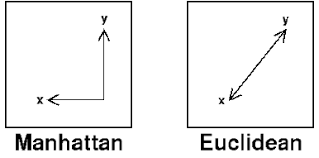
\includegraphics[width=4cm]{Figures/manhattan_euclidean.png}\\
    \end{center}
    
    {\color{cyan} Weighted Minkowski}: $d_{k}(a,b) = \sqrt[k]{\sum_{i=1}^{d}{w_{i}|a_{i}-b_{i}|^k}}$, in some scenarios, not all dimensions are equal. Can convey this idea using $w_{i}$. Generally not a good idea- should normalize data by Z-scores before computing distances.\\
    
    {\color{cyan} Cosine Similarity}: $cos(a,b) = \frac{a \cdot b}{|a||b|}$, calculates the similarity between 2 non-zero vectors, where $a \cdot b$ is the dot product (normalized between 0 and 1), higher values imply more similar vectors\\
    
    {\color{cyan} Kullback-Leibler Divergence}: $KL(A||B)=\sum_{i=i}^{d}{a_{i}log_{2}{\frac{a_{i}}{b_{i}}}}$\\
    KL divergence measures the distances between probability distributions by measuring the uncertainty gained or uncertainty lost when replacing distribution A with distribution B. However, this is not a metric but forms the basis for the Jensen-Shannon Divergence Metric.\\
    {\color{cyan} Jensen-Shannon}: $JS(A,B) = \frac{1}{2}KL(A||M)+ \frac{1}{2}KL(M||B)$, where M is the average of A and B. The JS function is the right metric for calculating distances between probability distributions 
    \end{minipage}
};
\node[fancytitle, right=10pt] at (box.north west) {Distance/Network Methods};
\end{tikzpicture}










% ------------------------------------------------------------------------
% ------------ Nearest Neighbor Classification -----------------
\begin{tikzpicture}
\node [mybox] (box){%
    \begin{minipage}{0.3\textwidth}
    \setlist{nolistsep}	

    
    Distance functions allow us to identify the points closest to a given target, or the \textit{nearest neighbors (NN)} to a given point. The advantages of NN include simplicity, interpretability and non-linearity.\\
    
    {\color{blue} \textbf{k-Nearest Neighbors}}\\
    Given a positive integer k and a point $x_{0}$, the KNN classifier first identifies k points in the training data most similar to $x_{0}$, then estimates the conditional probability of $x_{0}$ being in class $j$ as the fraction of the k points whose values belong to $j$. The optimal value for k can be found using cross validation.
    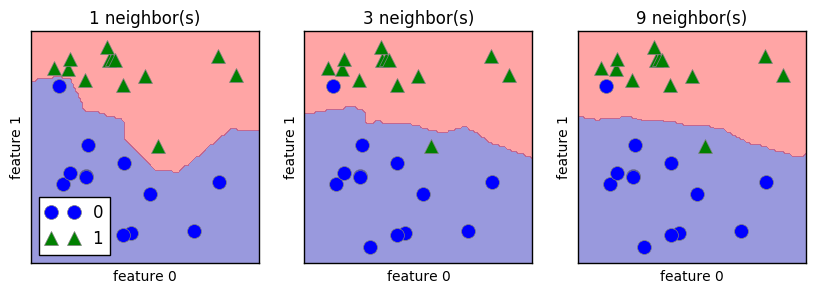
\includegraphics[width=\textwidth]{Figures/KNN.png}
    
    {\color{blue} \textbf{KNN Algorithm}}
    \begin{enumerate}
    	\item Compute distance D(a,b) from point b to all points 
        \item Select k closest points and their labels
        \item Output class with most frequent labels in k points 
    \end{enumerate}
    
    {\color{blue} \textbf{Optimizing KNN}}\\
    Comparing a query point a in d dimensions against n training examples computes with a runtime of $O(nd)$, which can cause lag as points reach millions or billions. Popular choices to speed up KNN include:
    \begin{itemize}
    	\item \textbf{Vernoi Diagrams}: partitioning plane into regions based on distance to points in a specific subset of the plane 
        \item \textbf{Grid Indexes}: carve up space into d-dimensional boxes or grids and calculate the NN in the same cell as the point
        \item \textbf{Locality Sensitive Hashing (LSH)}: abandons the idea of finding the exact nearest neighbors. Instead, batch up nearby points to quickly find the most appropriate bucket B for our query point. LSH is defined by a hash function $h(p)$ that takes a point/vector as input and produces a number/ code as output, such that it is likely that h(a) = h(b) if a and b are close to each other, and h(a)!= h(b) if they are far apart.
        
    \end{itemize}
    




    \end{minipage}
};
\node[fancytitle, right=10pt] at (box.north west) {Nearest Neighbor Classification};
\end{tikzpicture}
% ------------------------------------------------------------------------

% ------------ Clustering -----------------
\begin{tikzpicture}
\node [mybox] (box){%
    \begin{minipage}{0.3\textwidth}
    \setlist{nolistsep}	

	\textbf{Clustering} is the problem of grouping points by similarity using distance metrics, which ideally reflect the similarities you are looking for. Often items come from logical "sources" and clustering is a good way to reveal those origins. Perhaps the first thing to do with any data set. Possible applications include: hypothesis development, modeling over smaller subsets of data, data reduction, outlier detection.\\
    
    
    {\color{blue} \textbf{K-Means Clustering}}\\
    Simple and elegant algorithm to partition a dataset into K distinct, non-overlapping clusters. 
    \begin{enumerate}
    	\item Choose a K. Randomly assign a number between 1 and K to each observation. These serve as initial cluster assignments
        \item Iterate until cluster assignments stop changing
        \begin{enumerate}
        	\item For each of the K clusters, compute the cluster centroid. The kth cluster centroid is the vector of the p feature means for the observations in the kth cluster. 
            \item Assign each observation to the cluster whose centroid is closest (where closest is defined using distance metric).
        \end{enumerate}
    \end{enumerate}
    
    Since the results of the algorithm depends on the initial random assignments, it is a good idea to repeat the algorithm from different random initializations to obtain the best overall results. Can use MSE to determine which cluster assignment is better.\\
    
    {\color{blue} \textbf{Hierarchical Clustering}}\\
    Alternative clustering algorithm that does not require us to commit to a particular K. Another advantage is that it results in a nice visualization called a \textbf{dendrogram}. Observations that fuse at bottom are similar, where those at the top are quite different- we draw conclusions based on the location on the vertical rather than horizontal axis. 
    \begin{enumerate}
        \item Begin with n observations and a measure of all the $\frac{(n){n-1}}{2}$ pairwise dissimilarities. Treat each observation as its own cluster.
        \item For i = n, n-1, ...2
        	\begin{enumerate}
        		\item Examine all pairwise inter-cluster dissimilarities among the i clusters and identify the pair of clusters that are least dissimilar ( most similar). Fuse these two clusters. The dissimilarity between these two clusters indicates height in dendrogram where fusion should be placed. 
            	\item Assign each observation to the cluster whose centroid is closest (where closest is defined using distance metric).
        \end{enumerate}
    \end{enumerate}
    
    \textbf{Linkage}: Complete (max dissimilarity), Single (min), Average, Centroid (between centroids of cluster A and B)


    
%     \includegraphics[width=\textwidth]{}

    \end{minipage}
};
\node[fancytitle, right=10pt] at (box.north west) {Clustering};
\end{tikzpicture}


% ------------ Machine Learning -----------------
\begin{tikzpicture}
\node [mybox] (box){%
    \begin{minipage}{0.3\textwidth}
    \setlist{nolistsep}	

    
    {\color{blue} \textbf{Comparing ML Algorithms}}\\
    \textbf{Power and Expressibility}: ML methods differ in terms of complexity. Linear regression fits linear functions while NN define piecewise-linear separation boundaries. More complex models can provide more accurate models, but at the risk of overfitting.\\
    \textbf{Interpretability}: some models are more transparent and understandable than others (white box vs. black box models)\\
    \textbf{Ease of Use}: some models feature few parameters/decisions (linear regression/NN), while others require more decision making to optimize (SVMs)\\
    \textbf{Training Speed}: models differ in how fast they fit the necessary parameters\\
    \textbf{Prediction Speed}:  models differ in how fast they make predictions given a query\\
    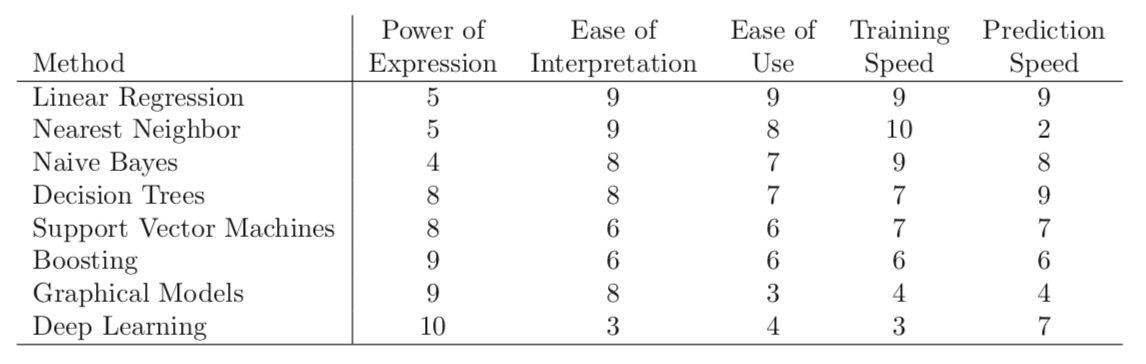
\includegraphics[width=\textwidth]{Figures/Comparing_Models.png}\\


    {\color{blue} \textbf{Naive Bayes}}\\
    Naive Bayes methods are a set of supervised learning algorithms based on applying Bayes’ theorem with the "naive" assumption of independence between every pair of features.\\
    
    \textbf{Problem}: Suppose we need to classify vector X = $x_{1}...x_{n}$ into $m$ classes, $C_{1}...C_{m}$. We need to compute the probability of each possible class given X, so we can assign X the label of the class with highest probability. We can calculate a probability using the Bayes' Theorem:

    $$ P(C_{i} | X) = \frac{P(X | C_{i}) P(C_{i})} {P(X)} $$
    
    Where:
    \begin{enumerate}
    	\item $P(C_{i})$: the prior probability of belonging to class $i$
		\item $P(X)$: normalizing constant, or probability of seeing the given input vector over all possible input vectors
		\item $P(X | C_{i})$: the conditional probability of seeing input vector X given we know the class is $C_{i}$\\
	\end{enumerate}

The prediction model will formally look like:
	\begin{center}
		$ C(X) = argmax_{i\in classes(t)}\ \frac{P(X | C_{i}) P(C_{i})} {P(X)} $
	\end{center}

where C(X) is the prediction returned for input X. 
    \end{minipage}
};
\node[fancytitle, right=10pt] at (box.north west) {Machine Learning Part I};
\end{tikzpicture}


% ------------ Machine Learning Part II -----------------
\begin{tikzpicture}
\node [mybox] (box){%
    \begin{minipage}{0.3\textwidth}
    \setlist{nolistsep}	

    
    {\color{blue} \textbf{Decision Trees}}\\
    Binary branching structure used to classify an arbitrary input vector X. Each node in the tree contains a simple feature comparison against some field ($x_{i} > 42$?). Result of each comparison is either true or false, which determines if we should proceed along to the left or right child of the given node. Also known as sometimes called classification and regression trees (CART).
    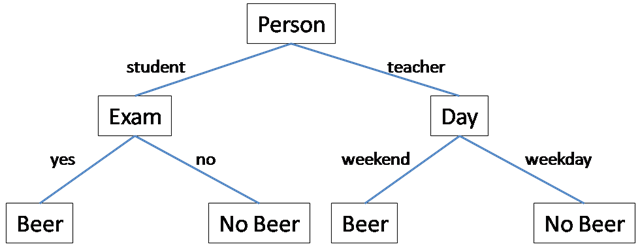
\includegraphics[width=\textwidth]{Figures/DecisionTree.png}
    
    \textbf{Advantages}: Non-linearity, support for categorical variables, easy to interpret, application to regression.\\
    \textbf{Disadvantages}: Prone to overfitting, instable (not robust to noise), high variance, low bias\\
    
    \textbf{\textit{Note}}: rarely do models just use one decision tree. Instead, we aggregate many decision trees using methods like ensembling, bagging, and boosting.\\
    
    {\color{blue} \textbf{Ensembles, Bagging, Random Forests, Boosting}}\\
    \textbf{Ensemble learning} is the strategy of combining many different classifiers/models into one predictive model. It revolves around the idea of voting: a so-called "wisdom of crowds" approach. The most predicted class will be the final prediction.\\
	\textbf{Bagging}: ensemble method that works by taking B bootstrapped subsamples of the training data and constructing B trees, each tree training on a distinct subsample as\\
    \textbf{Random Forests}: builds on bagging by decorrelating the trees. We do everything the same like in bagging, but when we build the trees, everytime we consider a split, a random sample of the p predictors is chosen as split candidates, not the full set (typically m $\approx$ $\sqrt{p}$). When m = p, then we are just doing bagging.\\
    \textbf{Boosting}: the main idea is to improve our model where it is not performing well by using information from previously constructed classifiers. Slow learner. Has 3 tuning parameters: number of classifiers B, learning parameter $\lambda$, interaction depth d (controls interaction order of model). 
    \end{minipage}
};
\node[fancytitle, right=10pt] at (box.north west) {Machine Learning Part II};
\end{tikzpicture}

% ------------ Machine Learning Part III -----------------
\begin{tikzpicture}
\node [mybox] (box){%
    \begin{minipage}{0.3\textwidth}
    \setlist{nolistsep}	

    
    {\color{blue} \textbf{Support Vector Machines}}\\
    Work by constructing a hyperplane that separates points between two classes. The hyperplane is determined using the maximal margin hyperplane, which is the hyperplane that is the maximum distance from the training observations. This distance is called the margin. Points that fall on one side of the hyperplane are classified as -1 and the other +1.
    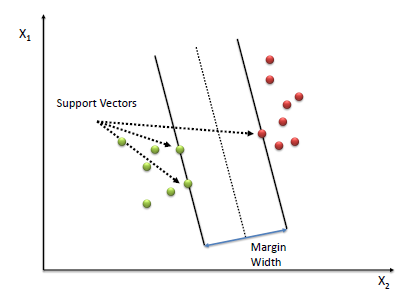
\includegraphics[width=\textwidth, height=3.5cm]{Figures/svm.png}
        
    
    {\color{blue} \textbf{Principal Component Analysis (PCA)}}\\
    \textbf{Principal components} allow us to summarize a set of correlated variables with a smaller set of variables that collectively explain most of the variability in the original set. Essentially, we are "dropping" the least important feature variables. \\
    
    \textbf{Principal Component Analysis} is the process by which principal components are calculated and the use of them to analyzing and understanding the data. PCA is an unsupervised approach and is used for dimensionality reduction, feature extraction, and data visualization. Variables after performing PCA are independent. Scaling variables is also important while performing PCA.
    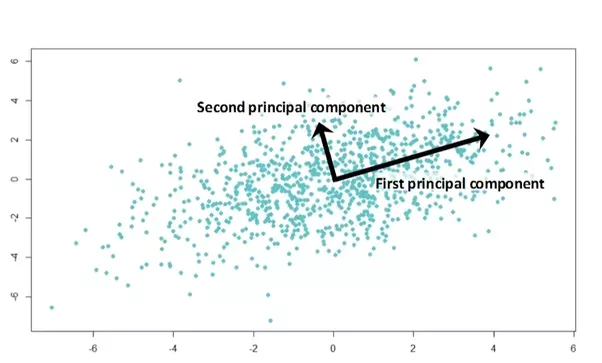
\includegraphics[width=\textwidth]{Figures/pca.png}

    \end{minipage}
};
\node[fancytitle, right=10pt] at (box.north west) {Machine Learning Part III};
\end{tikzpicture}


% ------------ Machine Learning Part IV -----------------
\begin{tikzpicture}
\node [mybox] (box){%
    \begin{minipage}{0.3\textwidth}
    \setlist{nolistsep}	
    
    {\color{blue}\textbf{ML Terminology and Concepts}}\\
    
	{\color{cyan} \textbf{Features}}: input data/variables used by the ML model\\ 
    {\color{cyan}\textbf{Feature Engineering}}: transforming input features to be more useful for the models. e.g. mapping categories to buckets, normalizing between -1 and 1, removing null\\ 
   	{\color{cyan}\textbf{Train/Eval/Test}}: training is data used to optimize the model, evaluation is used to asses the model on new data during training, test is used to provide the final result\\ 	
    {\color{cyan}\textbf{Classification/Regression}}: regression is prediction a number (e.g. housing price), classification is prediction from a set of categories(e.g. predicting red/blue/green)\\
    {\color{cyan}\textbf{Linear Regression}}: predicts an output by multiplying and summing input features with weights and biases\\
    {\color{cyan}\textbf{Logistic Regression}}: similar to linear regression but predicts a probability\\
    {\color{cyan}\textbf{Overfitting}}: model performs great on the input data but poorly on the test data (combat by dropout, early stopping, or reduce \# of nodes or layers)\\
    {\color{cyan}\textbf{Bias/Variance}}: how much output is determined by the features. more variance often can mean overfitting, more bias can mean a bad model \\
    {\color{cyan}\textbf{Regularization}}: variety of approaches to reduce overfitting, including adding the weights to the loss function, randomly dropping layers (dropout)\\
    {\color{cyan}\textbf{Ensemble Learning}}: training multiple models with different parameters to solve the same problem \\
    {\color{cyan}\textbf{A/B testing}}: statistical way of comparing 2+ techniques to determine which technique performs better and also if difference is statistically significant \\
    {\color{cyan}\textbf{Baseline Model}}: simple model/heuristic used as reference point for comparing how well a model is performing \\
    {\color{cyan}\textbf{Bias}}: prejudice or favoritism towards some things, people, or groups over others that can affect collection/sampling and interpretation of data, the design of a system, and how users interact with a system\\
    {\color{cyan}\textbf{Dynamic Model}}: model that is trained online in a continuously updating fashion\\
    {\color{cyan}\textbf{Static Model}}: model that is trained offline\\
    {\color{cyan}\textbf{Normalization}}:  process of converting an actual range of values into a standard range of values, typically -1 to +1\\
    {\color{cyan}\textbf{Independently and Identically Distributed (i.i.d)}}: data drawn from a distribution that doesn't change, and where each value drawn doesn't depend on previously drawn values; ideal but rarely found in real life\\
    {\color{cyan}\textbf{Hyperparameters}}: the "knobs" that you tweak during successive runs of training a model\\
    {\color{cyan}\textbf{Generalization}}: refers to a model's ability to make correct predictions on new, previously unseen data as opposed to the data used to train the model\\
    {\color{cyan}\textbf{Cross-Entropy}}: quantifies the difference between two probability distributions

    \end{minipage}
};

\node[fancytitle, right=10pt] at (box.north west) {Machine Learning Part IV};
\end{tikzpicture}


% ------------ Deep Learning Part I -----------------
\begin{tikzpicture}
\node [mybox] (box){%
    \begin{minipage}{0.3\textwidth}
    \setlist{nolistsep}	
    
    {\color{blue} \textbf{What is Deep Learning?}}\\
    Deep learning is a subset of machine learning. One popular DL technique is based on Neural Networks (NN), which loosely mimic the human brain and the code structures are arranged in layers. Each layer's input is the previous layer's output, which yields progressively higher-level features and defines a hierarchy. A Deep Neural Network is just a NN that has more than 1 hidden layer.
    
    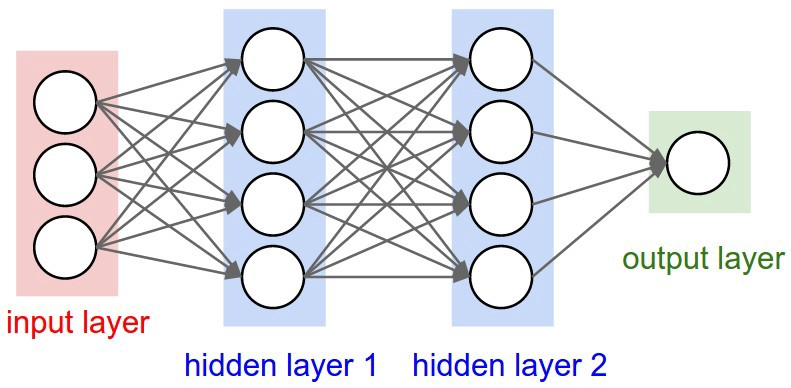
\includegraphics[width=\textwidth]{Figures/DL.jpeg}
    
    Recall that statistical learning is all about approximating $f(X)$. Neural networks are known as \textbf{universal approximators}, meaning no matter how complex a function is, there exists a NN that can (approximately) do the job. We can increase the approximation (or complexity) by adding more hidden layers and neurons.\\
    
     {\color{blue} \textbf{Popular Architectures}}\\
     There are different kinds of NNs that are suitable for certain problems, which depend on the NN's architecture.\\
     
    \textbf{Linear Classifier}: takes input features and combines them with weights and biases to predict output value\\
	\textbf{DNN}: deep neural net, contains intermediate layers of nodes that represent “hidden features” and activation functions to represent non-linearity\\ 
    \textbf{CNN}: convolutional NN, has a combination of convolutional, pooling, dense layers. popular for image classification. \\
    \textbf{Transfer Learning}: use existing trained models as starting points and add additional layers for the specific use case. idea is that highly trained existing models know general features that serve as a good starting point for training a small network on specific examples \\
    \textbf{RNN}: recurrent NN, designed for handling a sequence of inputs that have "memory" of the sequence. LSTMs are a fancy version of RNNs, popular for NLP\\
    \textbf{GAN}: general adversarial NN, one model creates fake examples, and another model is served both fake example and real examples and is asked to distinguish\\
    \textbf{Wide and Deep}: combines linear classifiers with deep neural net classifiers, "wide" linear parts represent memorizing specific examples and “deep” parts represent understanding high level features


    \end{minipage}
};
\node[fancytitle, right=10pt] at (box.north west) {Deep Learning Part I};
\end{tikzpicture}


% ------------ Deep Learning Part II -----------------
\begin{tikzpicture}
\node [mybox] (box){%
    \begin{minipage}{0.3\textwidth}
    \setlist{nolistsep}	 
        
   	{\color{blue} \textbf{Tensorflow}}\\
    Tensorflow is an open source software library for numerical computation using data flow graphs. Everything in TF is a graph, where nodes represent operations on data and edges represent the data. Phase 1 of TF is building up a computation graph and phase 2 is executing it. It is also distributed, meaning it can run on either a cluster of machines or just a single machine.  \\
    TF is extremely popular/suitable for working with Neural Networks, since the way TF sets up the computational graph pretty much resembles a NN.\\
    
      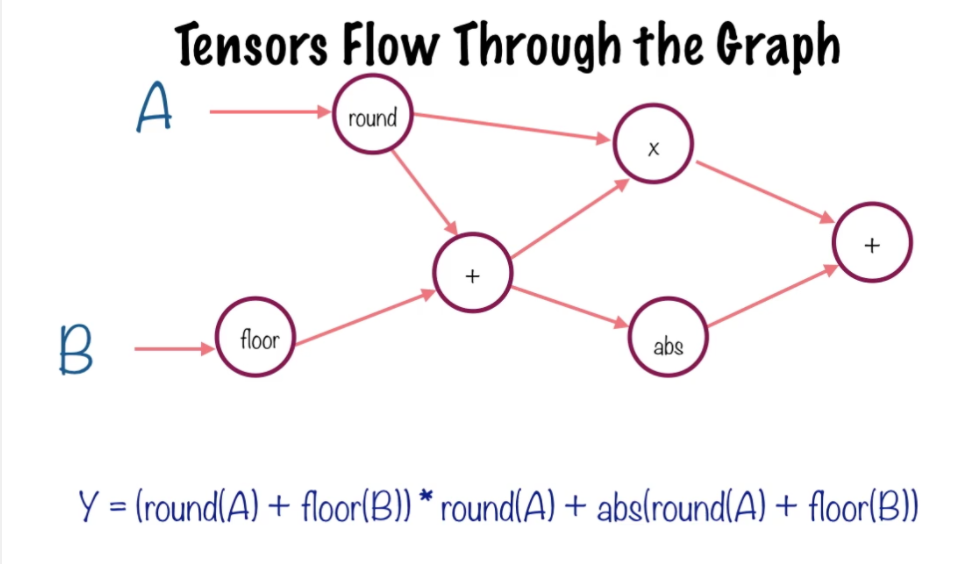
\includegraphics[width=\textwidth]{Figures/TF_DAG.png}
    
    
    {\color{blue} \textbf{Tensors}}\\
    In a graph, tensors are the edges and are multidimensional data arrays that flow through the graph. Central unit of data in TF and consists of a set of primitive values shaped into an array of any number of dimensions.\\
    A tensor is characterized by its rank (\# dimensions in tensor), shape (\# of dimensions and size of each dimension), data type (data type of each element in tensor).\\
    
    {\color{blue} \textbf{Placeholders and Variables}}\\
    \textbf{Variables}: best way to represent shared, persistent state manipulated by your program. These are the parameters of the ML model are altered/trained during the training process. Training variables. \\
    \textbf{Placeholders}: way to specify inputs into a graph that hold the place for a Tensor that will be fed at runtime. They are assigned once, do not change after. Input nodes
    
%     In ML, feature vectors are inputs/attributes which the ML algorithm focuses on. Each data point is a list (vector) of such vectors: aka feature vector. The output is a label or number.\\
%     Deep Learning is a representation ML based system that figures out by themselves what features to focus on. Neural networks are the most common class of deep learning algorithms, which are composed of neurons.
    \end{minipage}
};
\node[fancytitle, right=10pt] at (box.north west) {Deep Learning Part II};
\end{tikzpicture}

% ------------ Deep Learning Part III -----------------
\begin{tikzpicture}
\node [mybox] (box){%
    \begin{minipage}{0.3\textwidth}
    \setlist{nolistsep}	
    
    {\color{blue}\textbf{Deep Learning Terminology and Concepts}}\\
    
    {\color{cyan}\textbf{Neuron}}: node in a NN, typically taking in multiple input values and generating one output value, calculates the output value by applying an activation function (nonlinear transformation) to a weighted sum of input values\\
    {\color{cyan}\textbf{Weights}}: edges in a NN, the goal of training is to determine the optimal weight for each feature; if weight = 0, corresponding feature does not contribute\\
    {\color{cyan}\textbf{Neural Network}}: composed of neurons (simple building blocks that actually “learn”), contains activation functions that makes it possible to predict non-linear outputs\\
    {\color{cyan}\textbf{Activation Functions}}: mathematical functions that introduce non-linearity to a network e.g. RELU, tanh\\
    {\color{cyan}\textbf{Sigmoid Function}}: function that maps very negative numbers to a number very close to 0, huge numbers close to 1, and 0 to .5. Useful for predicting probabilities\\
    {\color{cyan}\textbf{Gradient Descent/Backpropagation}}: fundamental loss optimizer algorithms, of which the other optimizers are usually based. Backpropagation is similar to gradient descent but for neural nets \\
    {\color{cyan}\textbf{Optimizer}}: operation that changes the weights and biases to reduce loss e.g. Adagrad or Adam\\
    {\color{cyan}\textbf{Weights / Biases}}: weights are values that the input features are multiplied by to predict an output value. Biases are the value of the output given a weight of 0. \\
    {\color{cyan}\textbf{Converge}}: algorithm that converges will eventually reach an optimal answer, even if very slowly. An algorithm that doesn’t converge may never reach an optimal answer. \\
    {\color{cyan}\textbf{Learning Rate}}: rate at which optimizers change weights and biases. High learning rate generally trains faster but risks not converging, whereas a lower rate trains slower \\
        {\color{cyan}\textbf{Numerical Instability}}: issues with very large/small values due to limits of floating point numbers in computers\\
    {\color{cyan}\textbf{Embeddings}}: mapping from discrete objects, such as words, to vectors of real numbers. useful because classifiers/neural networks work well on vectors of real numbers\\
     {\color{cyan}\textbf{Convolutional Layer}}: series of convolutional operations, each acting on a different slice of the input matrix\\
     {\color{cyan}\textbf{Dropout}}: method for regularization in training NNs, works by removing a random selection of some units in a network layer for a single gradient step\\
     {\color{cyan}\textbf{Early Stopping}}: method for regularization that involves ending model training early\\     
    {\color{cyan}\textbf{Gradient Descent}}: technique to minimize loss by computing the gradients of loss with respect to the model's parameters, conditioned on training data\\
    {\color{cyan}\textbf{Pooling}}: Reducing a matrix (or matrices) created by an earlier convolutional layer to a smaller matrix. Pooling usually involves taking either the maximum or average value across the pooled area
    
%     \includegraphics[width=\textwidth]{}

    \end{minipage}
};
\node[fancytitle, right=10pt] at (box.north west) {Deep Learning Part III};
\end{tikzpicture}


%------------ Big Data- Hadoop Overview ---------------
\begin{tikzpicture}
\node [mybox] (box){%
    \begin{minipage}{0.3\textwidth}
    \setlist{nolistsep}	

    Data can no longer fit in memory on one machine (monolithic), so a new way of computing was devised using a group of computers to process this "big data" (distributed). Such a group is called a cluster, which makes up server farms. All of these servers have to be coordinated in the following ways: partition data, coordinate computing tasks, handle fault tolerance/recovery, and allocate capacity to process.\\
    
    {\color{blue} \textbf{Hadoop}}\\
    Hadoop is an open source \textit{distributed} processing framework that manages data processing and storage for big data applications running in clustered systems. It is comprised of 3 main components:
    \begin{itemize}
    	\item \textbf{Hadoop Distributed File System (HDFS)}: a distributed file system that provides high-throughput access to application data by partitioning data across many machines
        \item \textbf{YARN}: framework for job scheduling and cluster resource management (task coordination)
        \item \textbf{MapReduce}: YARN-based system for parallel processing of large data sets on multiple machines\\
	\end{itemize}

    {\color{blue} \textbf{HDFS}}\\
    Each disk on a different machine in a cluster is comprised of 1 master node and the rest are workers/data nodes. The \textbf{master node} manages the overall file system by storing the directory structure  and the metadata of the files. The \textbf{data nodes} physically store the data. Large files are broken up and distributed across multiple machines, which are also replicated across multiple machines to provide fault tolerance.\\
    
   {\color{blue} \textbf{MapReduce}}\\
   Parallel programming paradigm which allows for processing of huge amounts of data by running processes on multiple machines. Defining a MapReduce job requires two stages: map and reduce.
   
   \begin{itemize}
   	\item \textbf{Map}: operation to be performed in parallel on small portions of the dataset. the output is a key-value pair $<K,V>$
    \item \textbf{Reduce}: operation to combine the results of Map\\
   \end{itemize}
   
   {\color{blue} \textbf{YARN- Yet Another Resource Negotiator}}\\
   Coordinates tasks running on the cluster and assigns new nodes in case of failure. Comprised of 2 subcomponents: the resource manager and the node manager. The \textbf{resource manager} runs on  a single master node and schedules tasks across nodes. The \textbf{node manager} runs on all other nodes and manages tasks on the individual node.
    
%     A typical job process: the user defines defines the map and reduce tasks using MapReduce API, the job is triggered on the Hadoop cluster, YARN figures out where and how to run the job and stores the result in HDFS.

    \end{minipage};

};
\node[fancytitle, right=10pt] at (box.north west) {Big Data- Hadoop Overview};
\end{tikzpicture}


%------------ Big Data- Hadoop Ecosystem ---------------
\begin{tikzpicture}
\node [mybox] (box){%
    \begin{minipage}{0.3\textwidth}
    An entire ecosystem of tools have emerged around Hadoop, which are based on interacting with HDFS. Below are some popular ones:\\
    
    {\color{cyan} \textbf{Hive}}: data warehouse software built o top of Hadoop that facilitates reading, writing, and managing large datasets residing in distributed storage using SQL-like queries (HiveQL). Hive abstracts away underlying MapReduce jobs and returns HDFS in the form of tables (not HDFS). \\
    {\color{cyan} \textbf{Pig}}: high level scripting language (Pig Latin) that enables writing complex data transformations. It pulls unstructured/incomplete data from sources, cleans it, and places it in a database/data warehouses. Pig performs ETL into data warehouse while Hive queries from data warehouse to perform analysis (GCP: DataFlow).\\
    {\color{cyan} \textbf{Spark}}: framework for writing fast, distributed programs for data processing and analysis. Spark solves similar problems as Hadoop MapReduce but with a fast in-memory approach. It is an unified engine that supports SQL queries, streaming data, machine learning and graph processing. Can operate separately from Hadoop but integrates well with Hadoop. Data is processed using Resilient Distributed Datasets (RDDs), which are immutable, lazily evaluated, and tracks lineage. \\
    {\color{cyan} \textbf{Hbase}}: non-relational, NoSQL, column-oriented database management system that runs on top of HDFS. Well suited for sparse data sets (GCP: BigTable)  \\
    {\color{cyan} \textbf{Flink/Kafka}}: stream processing framework. Batch streaming is for bounded, finite datasets, with periodic updates, and delayed processing. Stream processing is for unbounded datasets, with continuous updates, and immediate processing. Stream data and stream processing must be decoupled via a message queue. Can group streaming data (windows) using tumbling (non-overlapping time), sliding (overlapping time), or session (session gap) windows. \\
    {\color{cyan} \textbf{Beam}}: programming model to define and execute data processing pipelines, including ETL, batch and stream (continuous) processing. After building the pipeline, it is executed by one of Beam’s distributed processing back-ends (Apache Apex, Apache Flink, Apache Spark, and Google Cloud Dataflow). Modeled as a Directed Acyclic Graph (DAG).\\
     {\color{cyan} \textbf{Oozie}}: workflow scheduler system to manage Hadoop jobs\\
     {\color{cyan} \textbf{Sqoop}}: transferring framework to transfer large amounts of data into HDFS from relational databases (MySQL)
    \end{minipage};
};
\node[fancytitle, right=10pt] at (box.north west) {Big Data- Hadoop Ecosystem};
\end{tikzpicture}



% ------------ SQL Part I -----------------
\begin{tikzpicture}
\node [mybox] (box){%
    \begin{minipage}{0.3\textwidth}
    Structured Query Language (SQL) is a declarative language used to access \& manipulate data in databases. Usually the database is a Relational Database Management System (RDBMS), which stores data arranged in relational database tables. A table is arranged in columns and rows, where columns represent characteristics of stored data and  rows represent actual data entries.\\

    {\color{blue} \textbf{Basic Queries}}\\
    - filter columns: \textbf{SELECT} col1, col3... \textbf{FROM} table1\\
	- filter the rows: \textbf{WHERE} col4 = 1 \textbf{AND} col5 = 2\\
	- aggregate the data: \textbf{GROUP BY}…\\
	- limit aggregated data: \textbf{HAVING} count(*) $>$ 1 \\
	- order of the results: \textbf{ORDER BY} col2\\
    
    Useful Keywords for \textbf{SELECT}\\
    \textbf{DISTINCT}- return unique results\\
	\textbf{BETWEEN} a AND b- limit the range, the values can be numbers, text, or dates\\
	\textbf{LIKE}- pattern search within the column text\\
	\textbf{IN} (a, b, c) - check if the value is contained among given\\
    
    {\color{blue} \textbf{Data Modification}}\\
    - update specific data with the \textbf{WHERE} clause: \\ \textbf{UPDATE} table1 \textbf{SET} col1 = 1 \textbf{WHERE} col2 = 2\\
    - insert values manually\\ \textbf{INSERT} \textbf{INTO} table1 (col1,col3) \textbf{VALUES} (val1,val3);\\
    - by using the results of a query\\ 
    \textbf{INSERT} \textbf{INTO} table1 (col1,col3) \textbf{SELECT} col,col2 FROM table2;\\
    
%     {\color{blue} \textbf{Views}}\\
%     A \textbf{VIEW} is a virtual table, which is a result of a query. Can be used to create virtual tables of complex queries.\\
% 	\textbf{CREATE VIEW} view1 \textbf{AS}\\
% 	\textbf{SELECT} col1, col2\\
% 	\textbf{FROM} table1\\
% 	\textbf{WHERE} …\\
    
    
    {\color{blue} \textbf{Joins}}\\
    The JOIN clause is used to combine rows from two or more tables, based on a related column between them.\\
    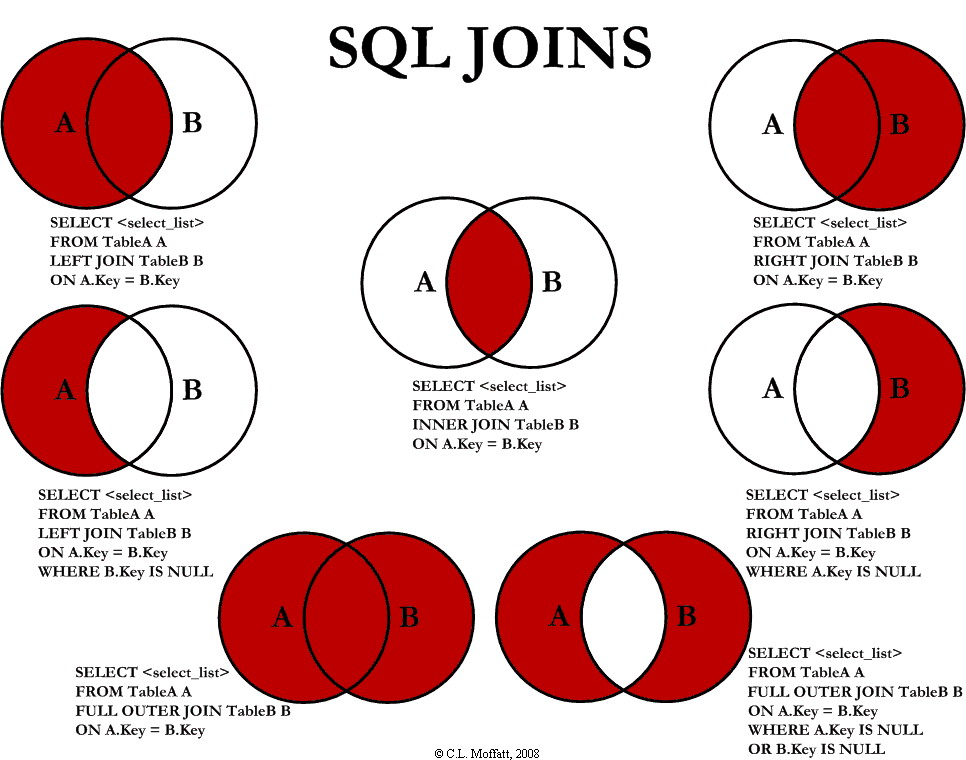
\includegraphics[width=\textwidth]{Figures/sql_joins.jpg}

    \setlist{nolistsep}	
    \end{minipage}
};
\node[fancytitle, right=10pt] at (box.north west) {SQL Part I};
\end{tikzpicture}




 
% ------------------------------------------------------------------------
% ------------ Recommended Resources -----------------
\begin{tikzpicture}
\node [mybox] (box){%
    \begin{minipage}{0.3\textwidth}
    \setlist{nolistsep}	

	\begin{itemize}
    	\item Data Science Design Manual\\
        (\url{www.springer.com/us/book/9783319554433)}
        \item Introduction to Statistical Learning \\
        (\url{www-bcf.usc.edu/~gareth/ISL/})
        \item Probability Cheatsheet \\(\url{/www.wzchen.com/probability-cheatsheet/})
        \item Google's Machine Learning Crash Course\\
        (\url{developers.google.com/machine-learning/crash-course/})
        
    \end{itemize}
    
%     \includegraphics[width=\textwidth]{}

    \end{minipage}
};
\node[fancytitle, right=10pt] at (box.north west) {Recommended Resources};
\end{tikzpicture}
% ------------------------------------------------------------------------



\end{multicols*}
\end{document}
Contact GitHub API Training Shop Blog About
© 2016 GitHub, Inc. Terms Privacy Security Status Help